\chapter{VLITE-Fast Pathfinder Survey}
\label{ch:data}

\par This chapter summaries the entirity of the data collected in numerous runs of the \vf system, and follows it up careful statistical analysis. All triggers from known sources are summarized.

\section {Campaign runs}
\label{sec:camp}

\par \vfpfs consists of data collected over multiple settings. 
Each campaign run is characterized by the type of filterbank data used (number of bits used for digitization) and the nature of trigger cuts used. 
This characterization breaks the whole of \vfpfs into multiple campaigns. 
Firstly, all the campaign runs are enumerated and discussed in brief before delving into the details in respective sub-sections.
\begin{description}
	\item[NBIT = 2 (NB2)] \\
		This was the first run of \vfpfs system. All the filterbank data was digitized to $2$ bits to test the computational capabilities of the pipeline. Conservative trigger cuts were employed for the same reason.
	\item[NBIT = 8 (NB8)] \\
		The filterbank data bit depth was increased to $8$ in this run. The trigger cuts were somewhat increaesd before.
	\item[Max Warp (MW)] \\
		The filterbank was digitized to $8$ bits same as before.
		The trigger cuts were drastically changed to be the most aggressive possible. 
\end{description}

The key features are summarized in ~\autoref{tab:campaigns}.

% Please add the following required packages to your document preamble:
% \usepackage{booktabs}
\begin{table}[]
	\label{tab:campaigns}
	\begin{tabular}{@{}llllllll@{}}
		\toprule
		Label & \begin{tabular}[c]{@{}l@{}}Start\\ (YYYY-MM-DD)\end{tabular} & \begin{tabular}[c]{@{}l@{}}End\\ (YYYY-MM-DD)\end{tabular} & \begin{tabular}[c]{@{}l@{}}On-sky\\ (day)\end{tabular} & \begin{tabular}[c]{@{}l@{}}Uptime\\ (\%)\end{tabular} & Triggers & \begin{tabular}[c]{@{}l@{}}Rate\\ (/hr)\end{tabular} & Comments \\ \midrule
		NB2 & 2019-10-17 & 2019-12-05 & 27.03 & 55.61 & 10 306 & 15.89 & Two bit digitization \\
		NB8 & 2019-12-19 & 2020-01-21 & 12.16 & 36.10 & 12 028 & 41.19 & Eight bit digitization with more lower trigger cuts \\
		MW & 2020-01-22 & 2020-06-27 & 87.16 & 55.32 & 826 294 & 394.85 & Eight bit digitization with the minimum possible trigger cuts \\
		ALL & 2019-10-17 & 2020-06-27 & 126.38 & 49.79 & 848 628 & 279.77 & All the campaigns \\ \bottomrule
	\end{tabular}
	\caption{Salient features of the campaign runs.}
\end{table}

\subsection {NB2}

\par In an epoch from \texttt{2019-10-17} to \texttt{2019-12-05} spanning for $49$ days, \vf was onsky for $27.03$ days. 
This resulted in capturing $10\ 306$ triggers, yielding a trigger rate of $\sim 16\ {\rm hr}^{-1}$. The uptime achieved in this was $55.6\%$.
The main features of this run was that the data was digitized to \nbit{2} hence the name. 
The trigger cuts were humble:
\begin{align*}
	{\rm S/N} &\geq 8 \\
	{\rm DM} &\geq 50 {\rm\ pc/cc} \\
	{\rm Width} &\leq 100 {\rm\ ms}
\end{align*}

\par This run didn't have the \dbson trigger mechanics in place. Instead, for every trigger \fbson~ files were written to disks at all the antennas including the coadded antenna as well.

\subsection {NB8}

\par In an epoch from from \texttt{2019-12-19} to \texttt{2020-01-21}spanning $33$ days, \vf was onsky for $12.16$ days.
During which, \vf~ collected $12\ 028$ triggers, yielding an event rate of $\sim 41\ {\rm hr}^{-1}$.
Fraction of total time spent on sky was $36.10\%$. 
The trigger cuts were a bit more agressive than NB2 run.
\begin{align*}
	{\rm S/N} &\geq 7.5 \\
	{\rm DM} &\geq 50 {\rm\ pc/cc} \\
	{\rm Width} &\leq 100 {\rm\ ms}
\end{align*}


\subsection {MW}

\par This is the longest campaign run in the \vfpfs. 
Starting from \texttt{2020-01-22} to \texttt{2020-06-27}, in a total length of $157$ days, \vf~ achieved $55.32$ uptime by being on sky for $\sim 87$ days.
Two separate trigger cuts were employed to keep trigger rates in check.
The trigger cuts were as aggressive as possible, hence, collecting $826\ 294$ triggers with trigger rate of $\sim 395\ {\rm hr}^{-1}$.
\begin{align*}
	{\rm S/N} &\geq 6.0 \&  {\rm S/N} &\geq 8.0 \\
	{\rm DM} &\geq 50 {\rm\ pc/cc}  \& {\rm DM} &\geq 50 {\rm\ pc/cc}\\
	{\rm Width} &\leq 100 {\rm\ ms} \& {\rm Width} &\in [20, 100] {\rm\ ms}
\end{align*}

\section {Detection of pulsars}

\par A large onsky time yields many serendiptious triggers caused by pulses from pulsars. 
These detections are a field test for \vf and are tabulated in~\autoref{tab:psrdetect}.
Based on these detections, a rudimentary argument for Field of View (FOV) (~\autoref{ssub:fov}) and sensitivity (~\autoref{ssub:sensitiviy})is formulated.

% Please add the following required packages to your document preamble:
% \usepackage{booktabs}
\begin{table}[]
	\label{tab:psrdetect}
	\begin{tabular}{@{}lllllllll@{}}
		\toprule
		PSRJ & \begin{tabular}[c]{@{}l@{}}RAJ\\ (hh:mm:ss)\end{tabular} & \begin{tabular}[c]{@{}l@{}}DECJ\\ (dd:mm:ss)\end{tabular} & \begin{tabular}[c]{@{}l@{}}DM\\ (pc/cc)\end{tabular} & \begin{tabular}[c]{@{}l@{}}P0\\ (s)\end{tabular} & \begin{tabular}[c]{@{}l@{}}W50\\ (ms)\end{tabular} & N & \begin{tabular}[c]{@{}l@{}}S400\\ (mJy)\end{tabular} & \begin{tabular}[c]{@{}l@{}}Time on source\\ (hr)\end{tabular} \\ \midrule
		J1752-2806 & 17:52:58.6 & -28:06:37.3 & 50.37 & 0.562 & 6.1 & 2196 & 1100.0 & 2.00 \\
		J0534+2200 & 05:34:31.9 & +22:00:52.0 & 56.77 & 0.033 & 3.0 & 24 & 550.0 & 0.84 \\
		J1745-3040 & 17:45:56.3 & -30:40:22.9 & 88.37 & 0.367 & 6.1 & 29 & 66.0 & 23.72 \\
		J2321+6024 & 23:21:55.2 & +60:24:31 & 94.59 & 2.256 & 131.1 & 4 & 36.0 & 0.14 \\
		J1935+1616 & 19:35:47.8 & +16:16:39.9 & 158.52 & 0.358 & 6.0 & 34 & 242.0 & 1.72 \\
		J1922+2110 & 19:22:53.5 & +21:10:42 & 217.09 & 1.077 & 14.8 & 10 & 30.0 & 9.70 \\ \bottomrule
	\end{tabular}
\caption {Observed pulsars}
\end{table}

\begin{figure}
	\centering
	\label{fig:psrdetect}
	\caption{Collage of averaged pulses from the detected pulsars.}
\end{figure}

\subsection{Field of View}
\label{ssub:fov}

\par It is worthwhile to understand the spatial extent over which the \psr{J1752} (from now on dm50) has been detected. 
This exercise would help us visualize how large of a field-of-view \vf posses.
Angular resolution on the basis of a diffraction limit arguments is $\sim 2^o$ (c.f.~\autoref{ssub:vfrb}).
See ~\autoref{fig:dm50fov}. 
\begin{figure}
	\label{fig:dm50fov}
	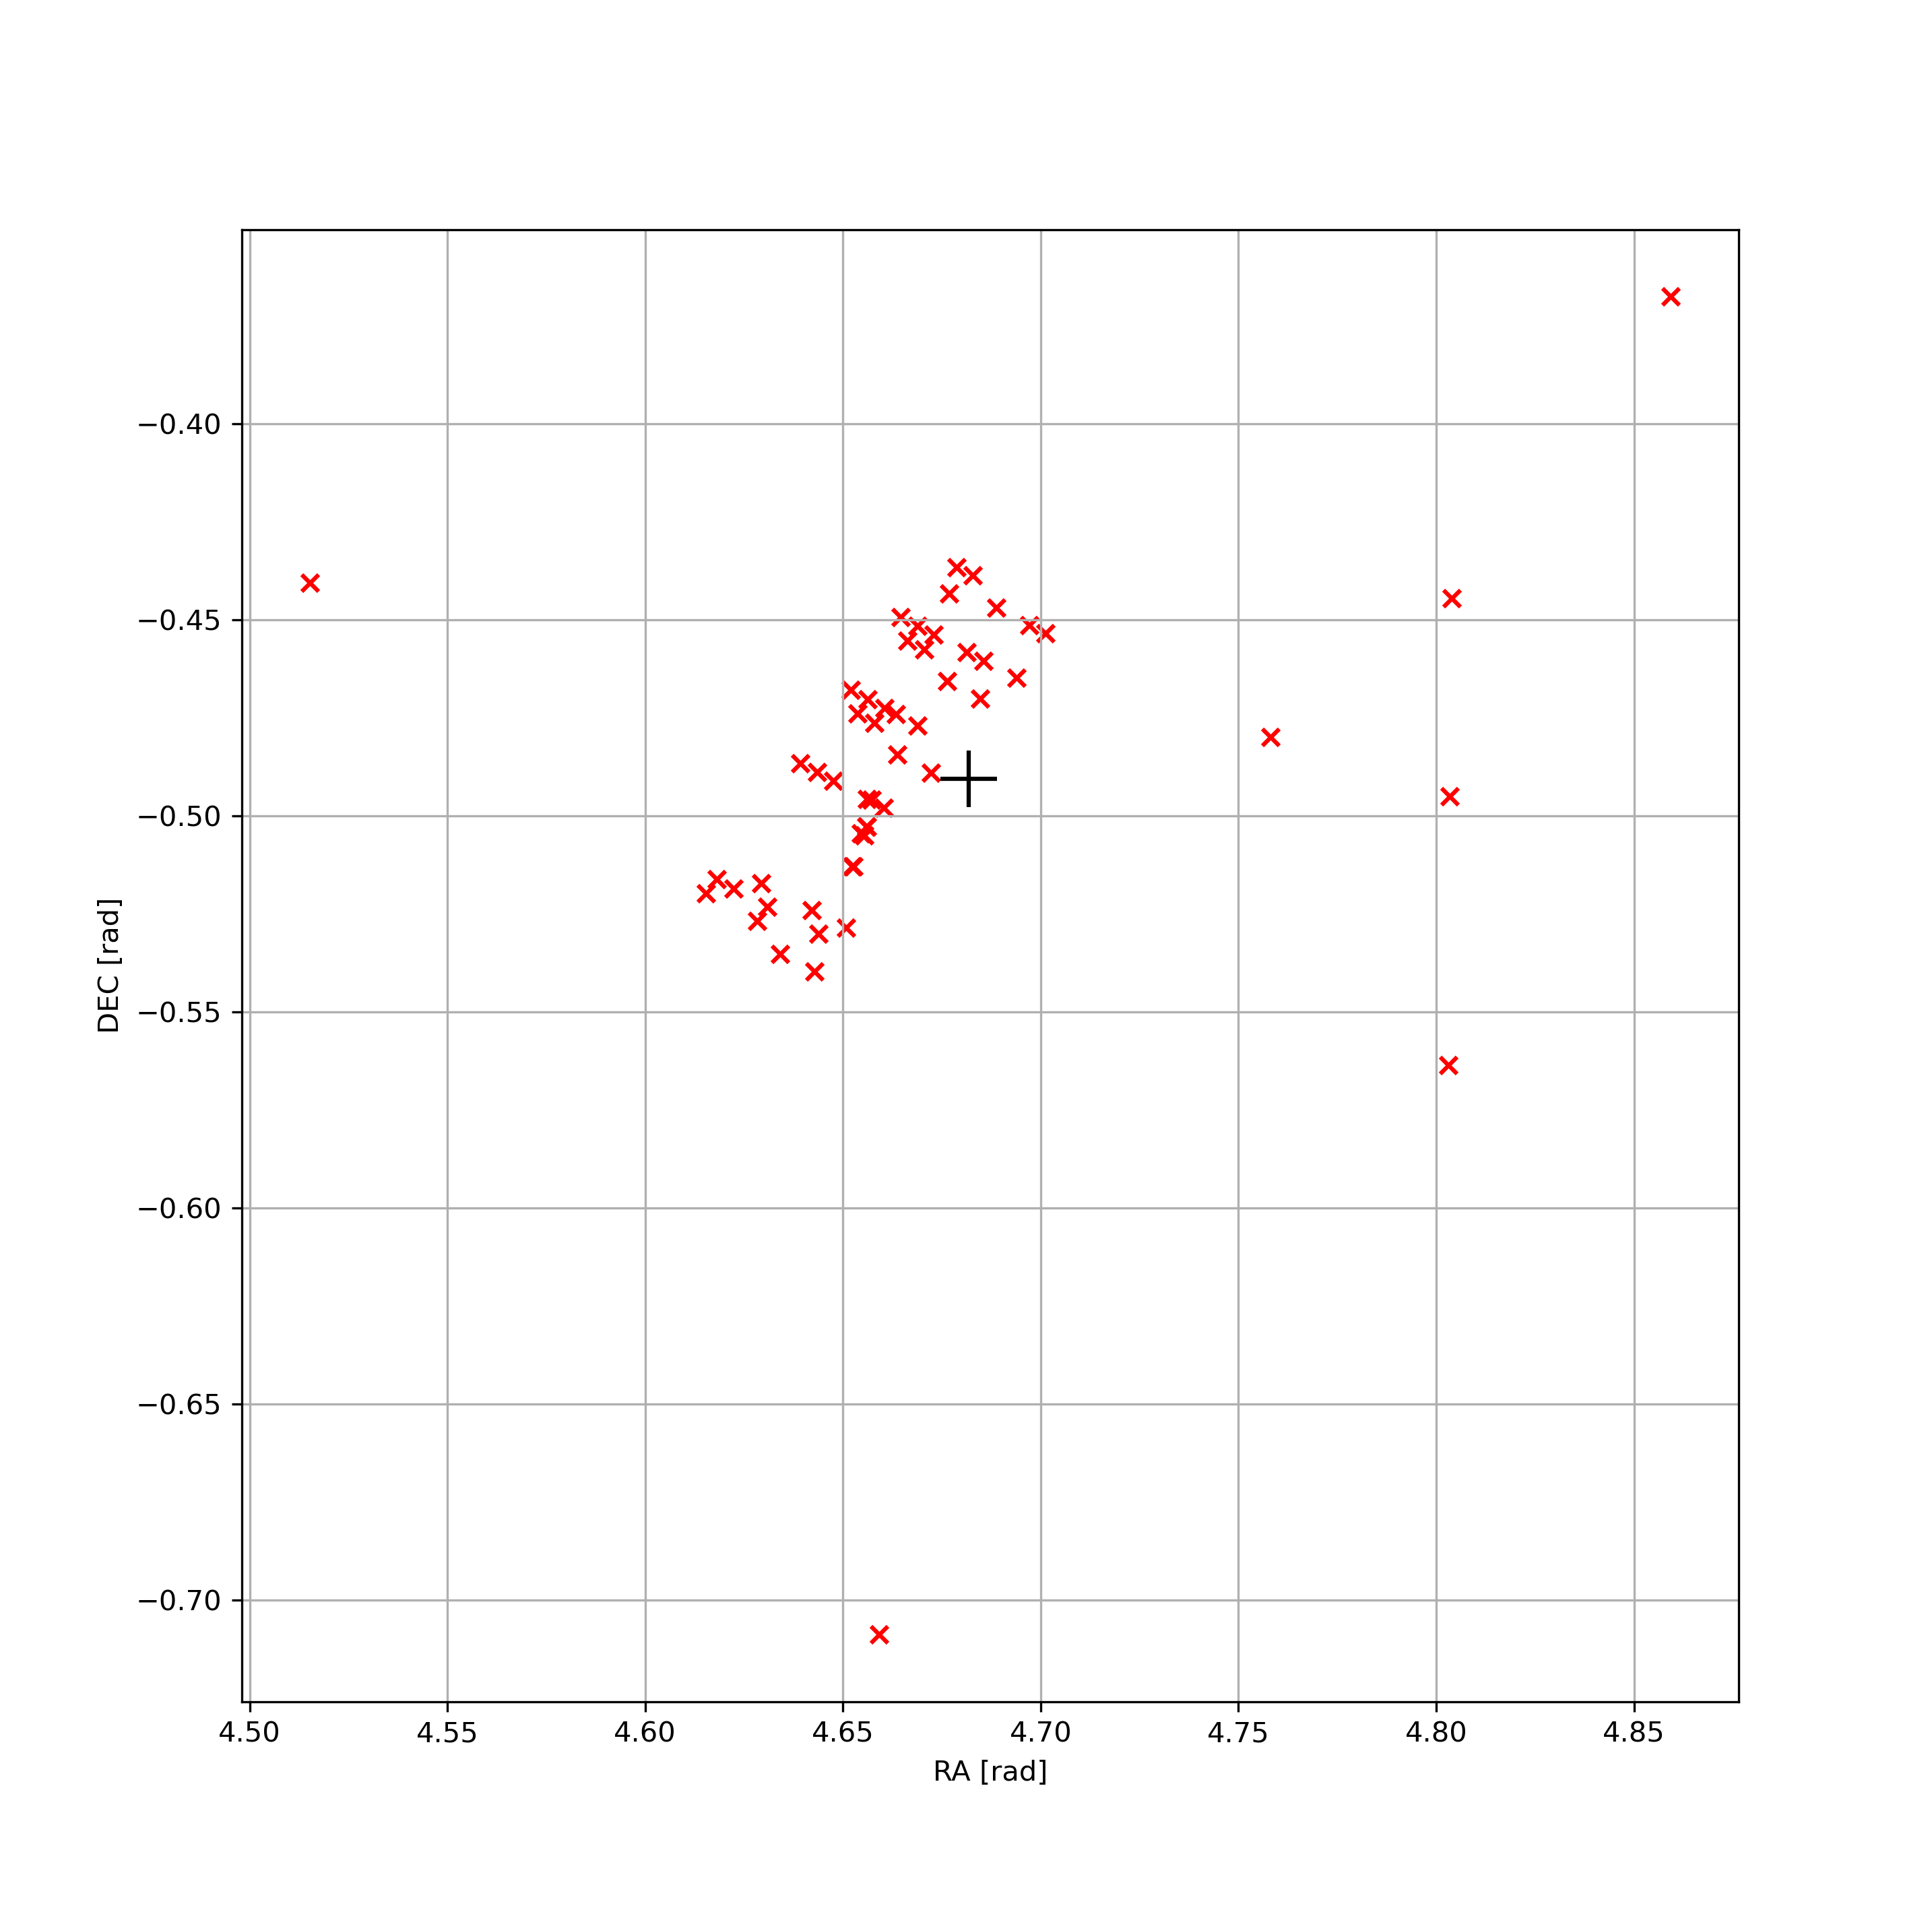
\includegraphics[width=0.8\textwidth, keepaspectratio]{dm50_fov.png}
	\caption{Large FOV of \vf understood using \psr{J1752-2806} as a marker. 
	Dots represent the pointings where triggers from the pulsars were recorded.
	%Numbers next to the dots represent fraction of the total number of triggers detected at the pointing.
	%Overlayed dashed lines represent angular size of $2"$ (in red).
}
\end{figure}

\subsection {Sensitivity}
\label{ssub:sensitiviy}

\par The sensitivity of the \vf can be understood using the detected set of pulsars.
Since, each pulsar has a documented flux density at $400$ MHz, available in \texttt{PSRCAT}(~\cite{psrcat}).
With the help of number of pulses detected, the sensitivity of \vf~ can be loosely extrapolated on the basis of the pulsars.

\begin{figure}
	\label{fig:psrs400}
	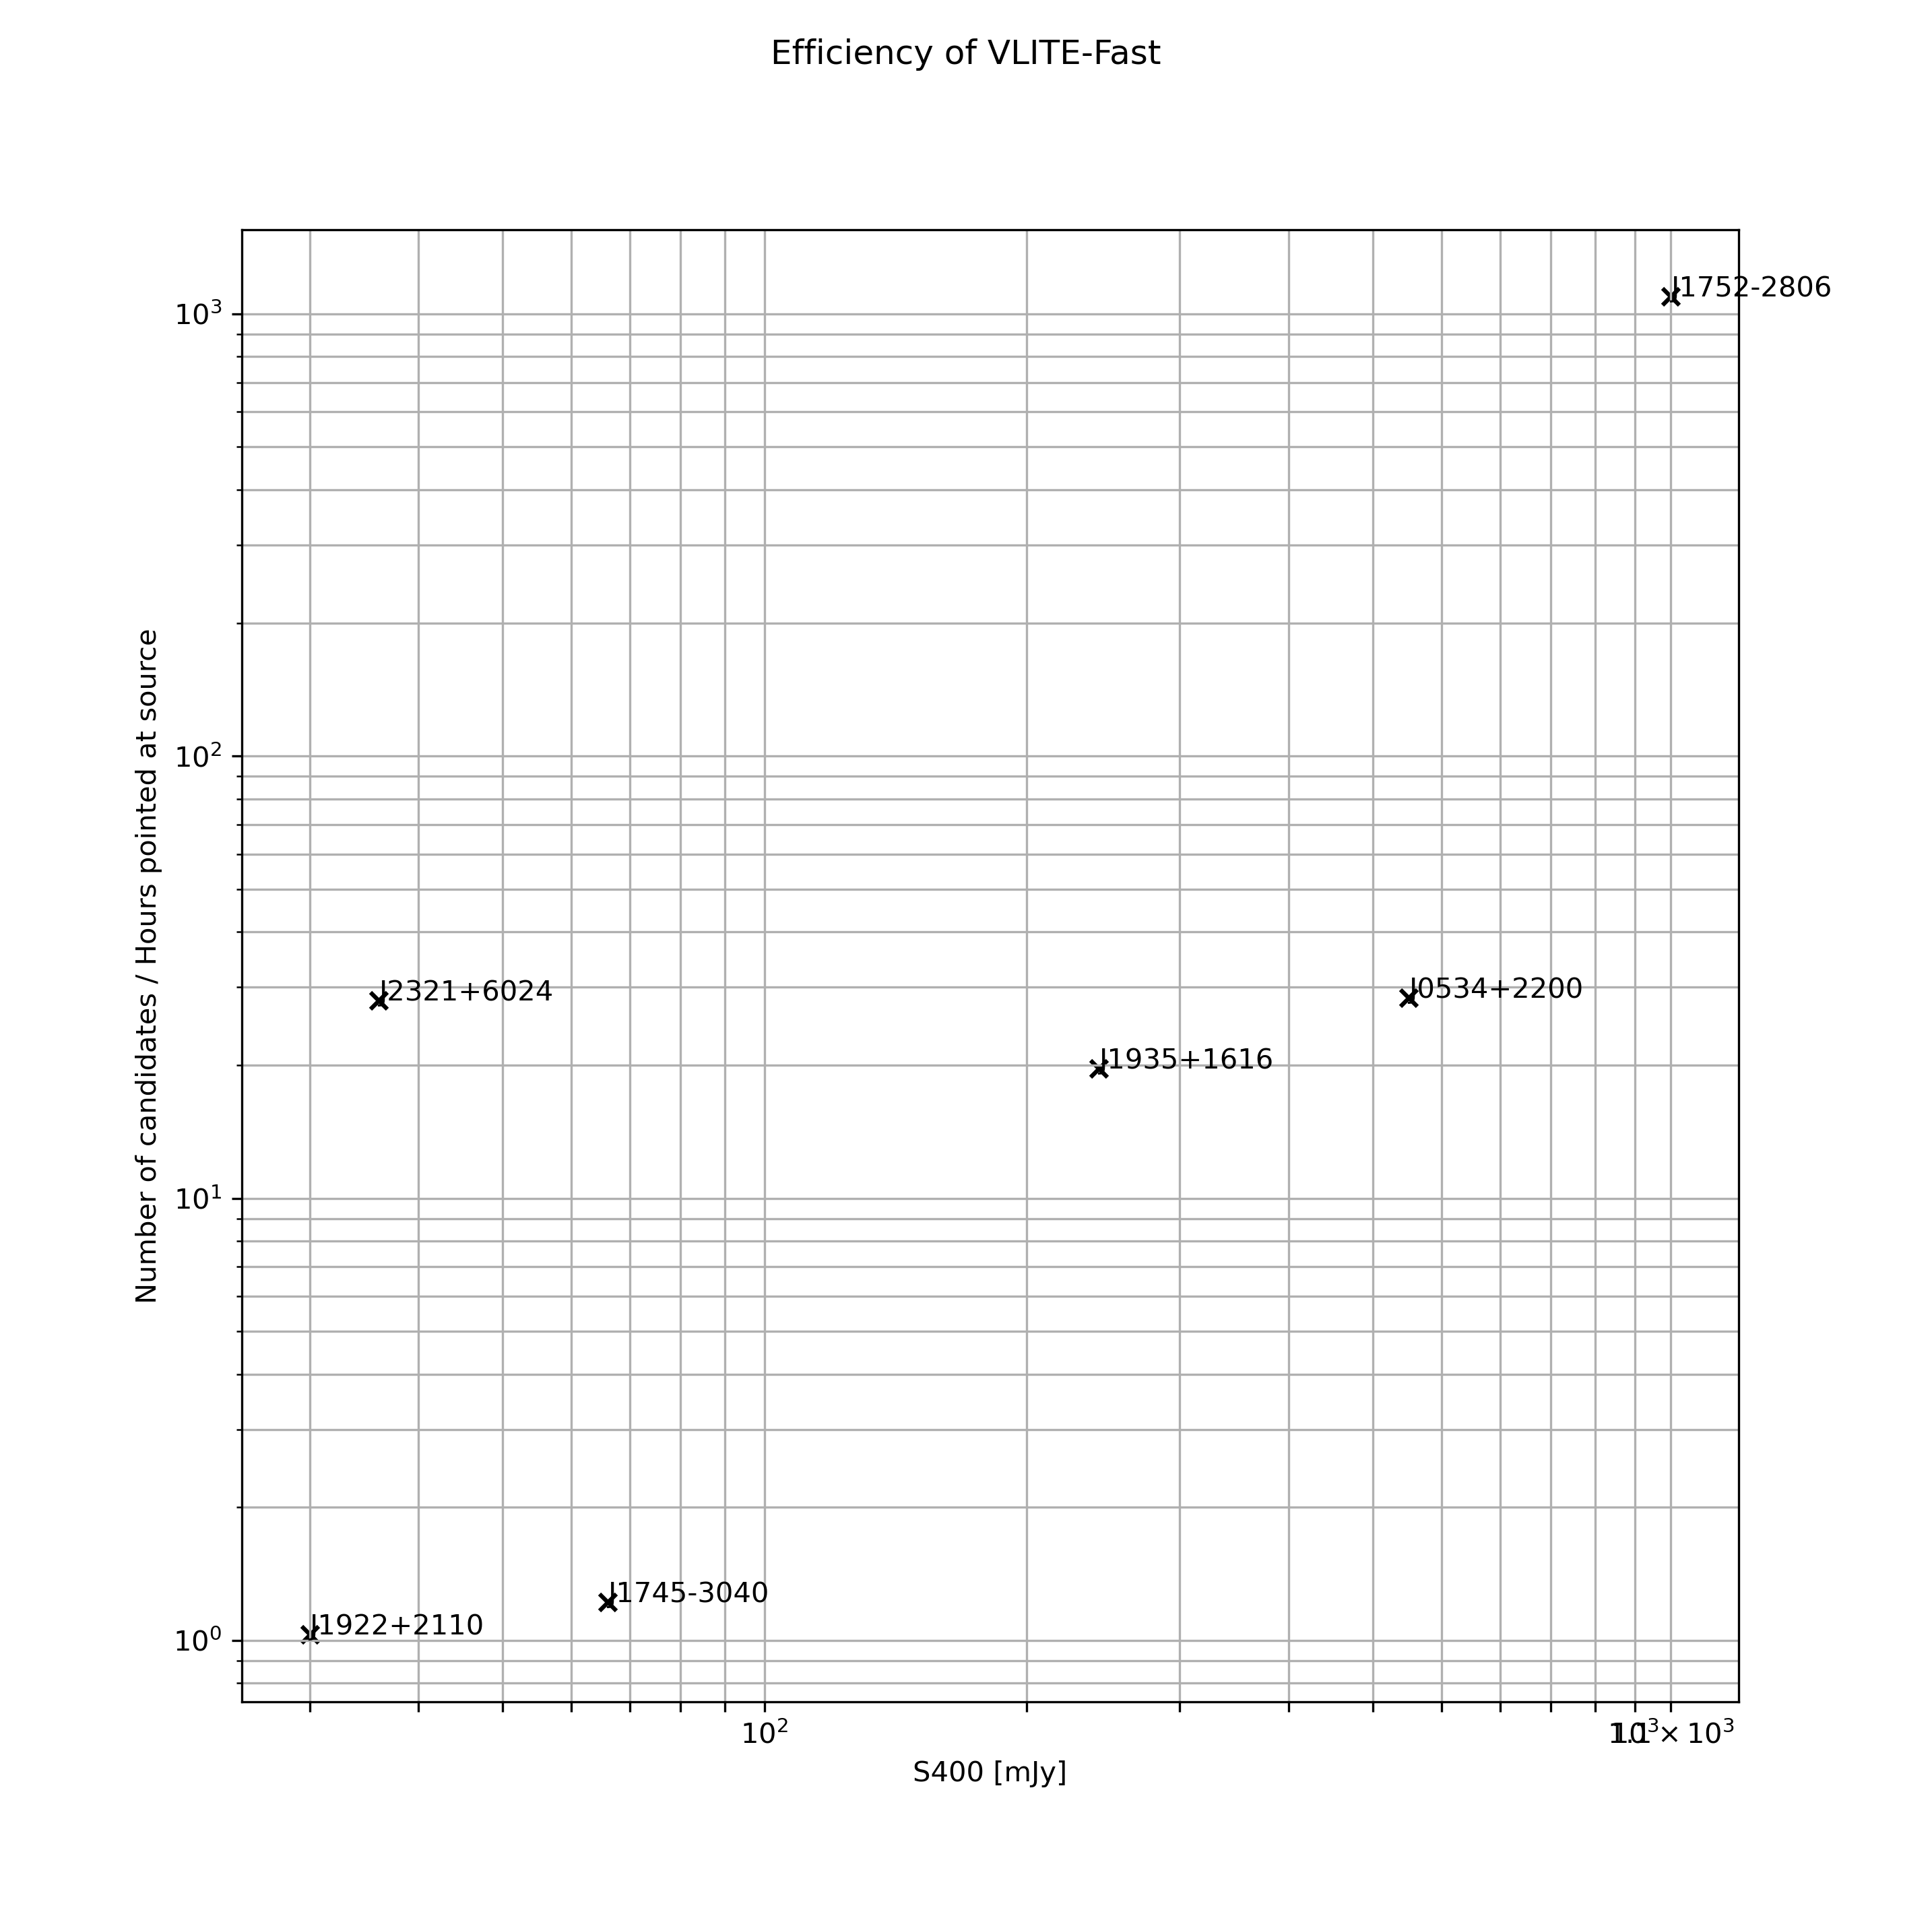
\includegraphics[width=0.8\textwidth, keepaspectratio]{psr_efficiency.png}
	\caption{Sensitivity of \vf using triggers from pulsars and documented flux density. 
		Flux density is plotted on x-axis. Triggers received divided by time spent on sky is plotted on the y-axis.
	}
\end{figure}
\section {RFI}
\label{sec:RFI}

\par One of the major challenges any radio observatory faces is that of Radio Frequency Interference (RFI). 
These are spurious radio signals of human origin polluting the frequency band of interest. In a search pipeline such as \vf, 
RFI causes large number of triggers which tax the pipeline. 
One of the main reasons for \vf pipeline failing from time to time is the lag caused by serving many spurious triggers because of RFI.
Naturally, with the triggers collected so far, a strategy can be devised to understand the triggers caused by RFI and mitigate them realtime.
This is described in~\autoref{ssub:rfim}. \vfpfs also observed recurring RFI which produces a distinct feature in the \dm~ distribution. This artifact is discussed in~\autoref{ssub:dm150}.

\subsection {RFI contamination}
\label{ssub:rfim}

\par Detection of a true signal (of astrophysical origin) is a rare occasion. Registering a large number of triggers in a short time is indicative of RFI.
This fact is used to measure the amount of RFI contamination in the \vfpfs data.
All the triggers are collected in $8$-second batches and counted.
If a given batch has a large number of triggers in it, it is treated as RFI.
Figuring out the correct \emph{large} number of triggers is done heuristically.

\par Firstly, the cumulative distribution of the number of triggers in a batch (of $8$ seconds) is computed. See~\autoref{fig:rficon}.
Understanding that RFI would only be contaminating a small percent of the whole data. 
One would expect the cumulative distribution to flatten out for larger number of triggers in a batch.
Another way to interpret the same would be that only a small portion of the dataset have extremely high trigger activity.
A suitable threshold is thus selected which limits the maximum number of triggers in a batch of $8$ seconds but retains most of the triggers.
Mathematically, this threshold which be an inflection point of the cumulative distribution function.

\begin{figure}
	\label{fig:rficon}
	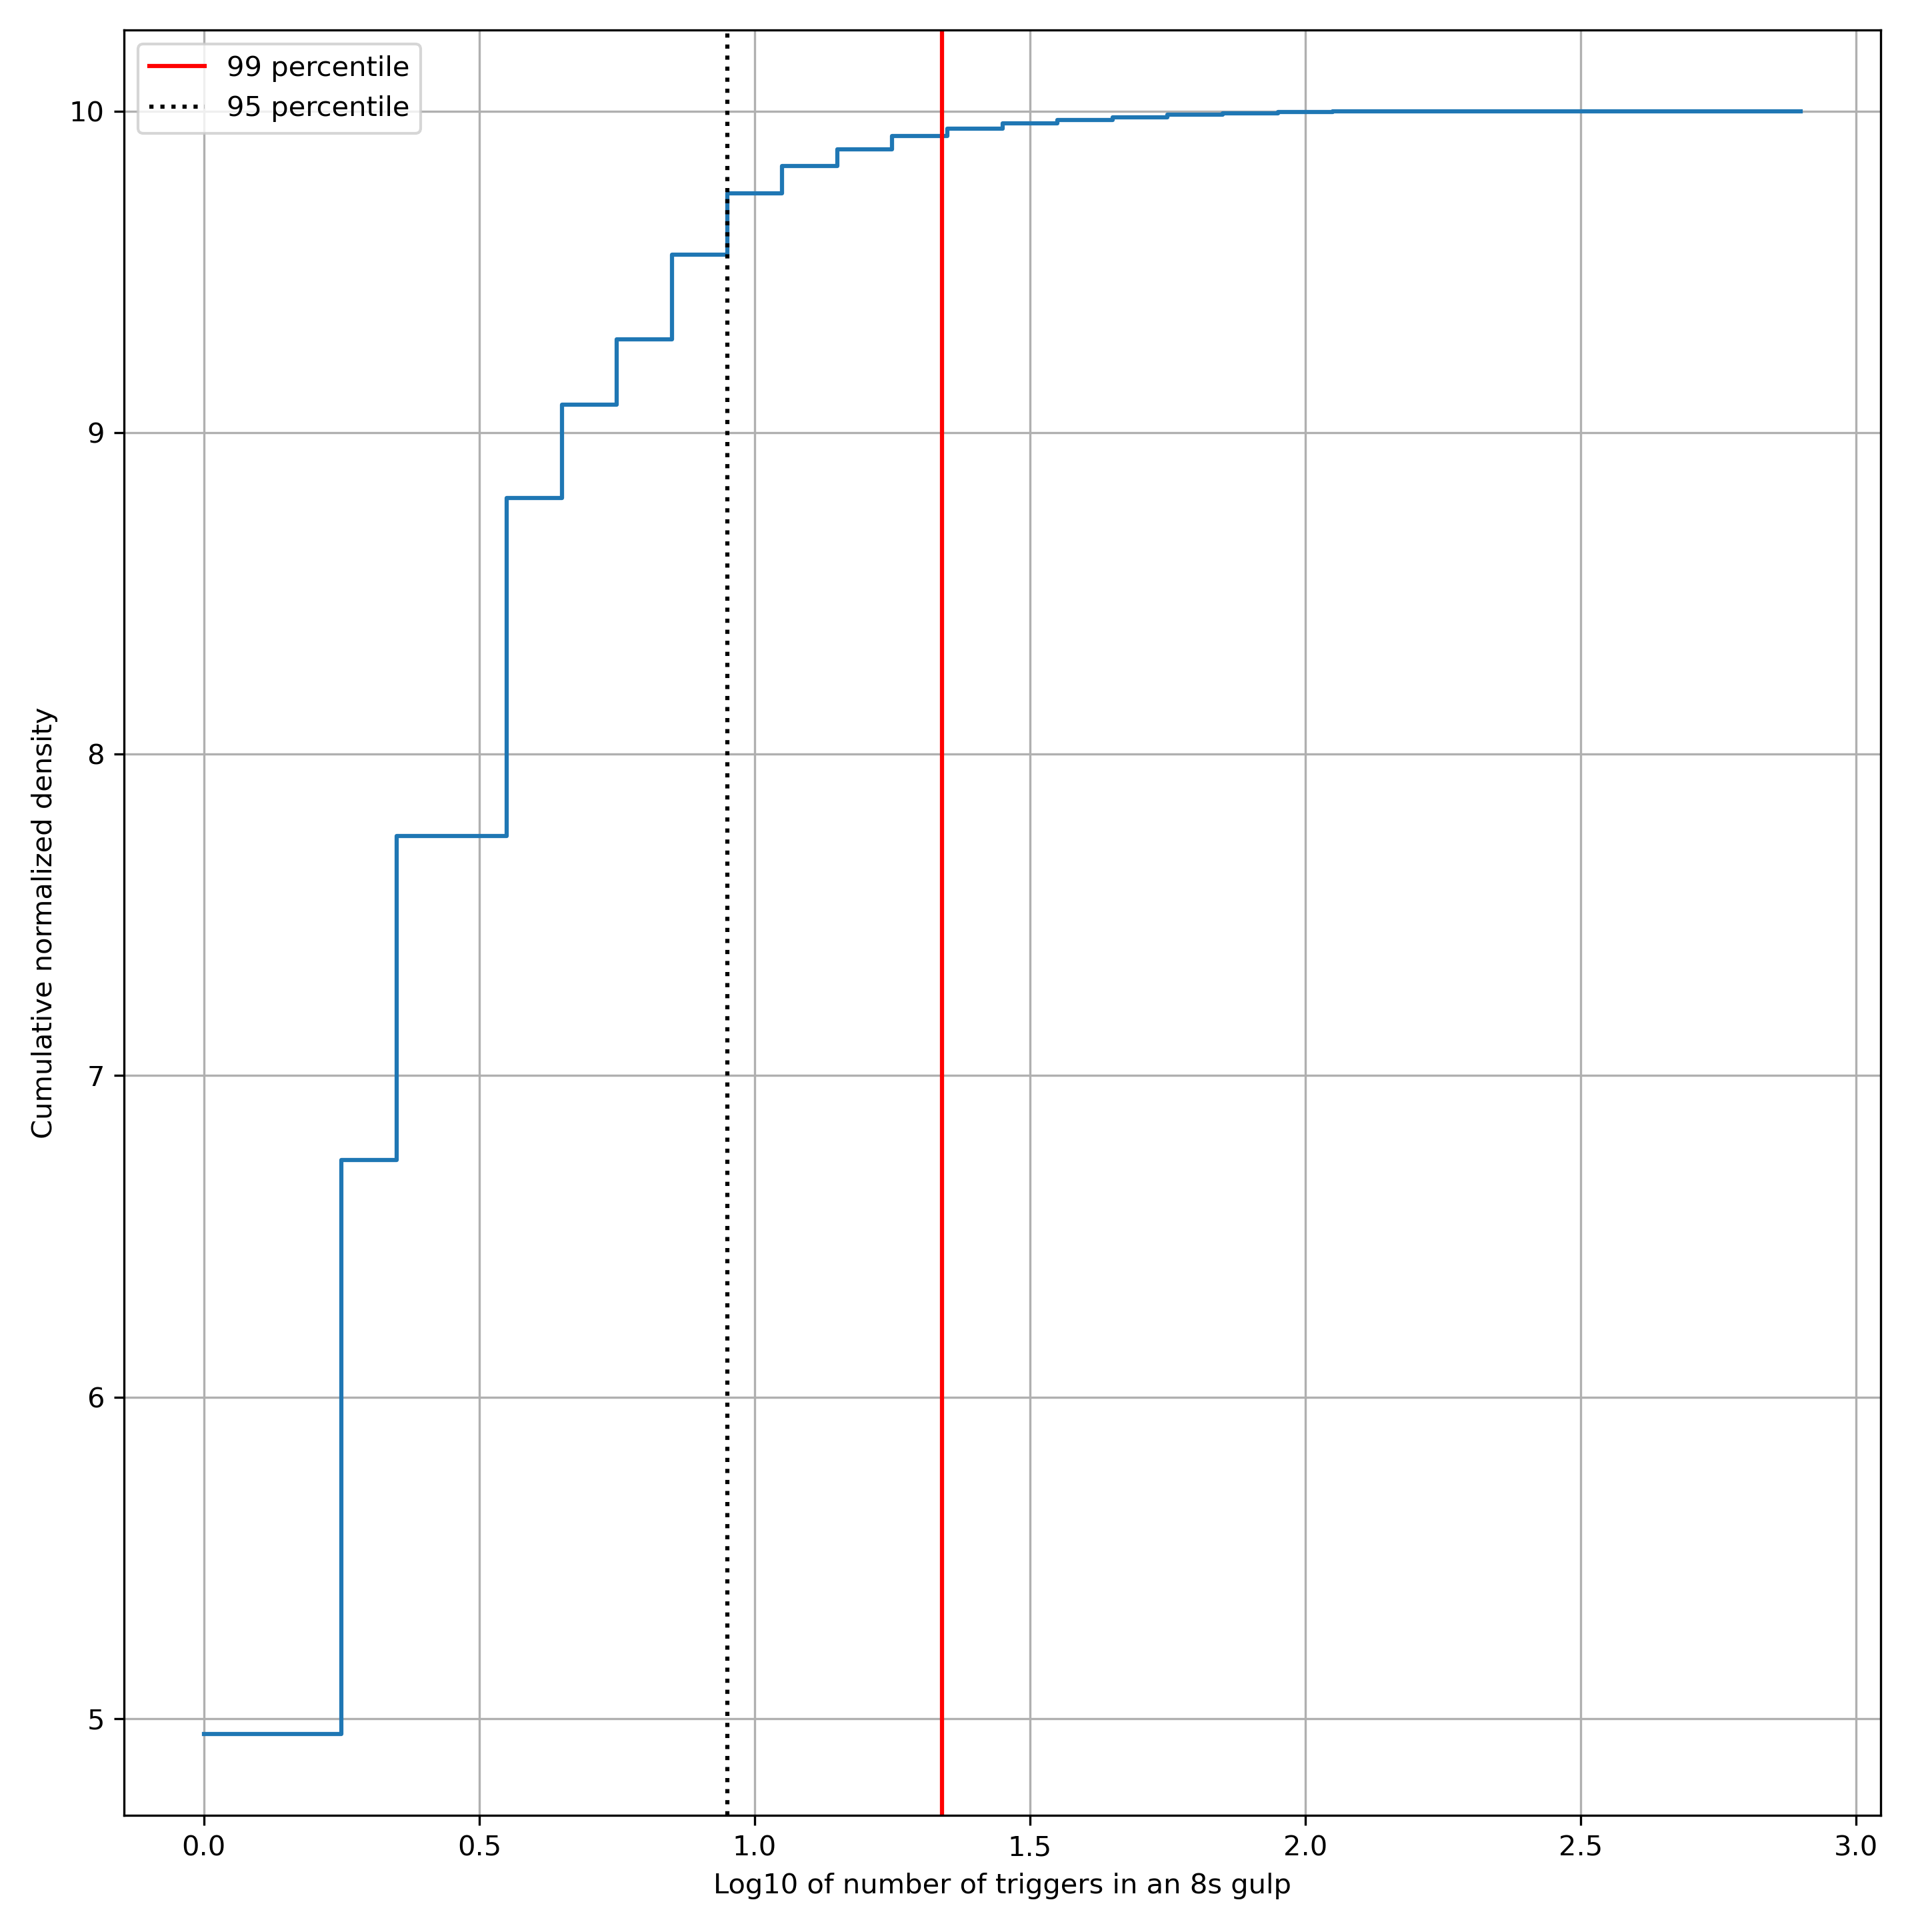
\includegraphics[width=0.8\textwidth, keepaspectratio]{rficum.png}
	\caption{Cumulative distribution of number of candidates received in an $8$-second gulp.
		Setting a limit of $10$ candidates in a gulp, and treating the rest as RFI gulps, $\sim1\%$ of the \vfpfs data is said to be contaminated with RFI.
	}
\end{figure}

\subsection {\DM{150} artifact}
\label{ssub:dm150}

\par Short time RFI in a single frequency channel does not produce spurious triggers since bandpass normalization on the time windown containing the RFI cancels its intensity. 
However, when there is short time RFI in separate channels, it is a different story. 
If such a short time RFI is coincident in time, any search pipeline would register it as a \DM{0} signal and can be filtered out easily.
But, if the same RFI has a time offset between the frequency channels, it causes the same search pipeline to register spurious triggers and are much more difficult to excise.

\par A short time RFI exisiting only in specific frequency channels having time offset between the channels behaves like a dispersed signal. 
And a candidate is registered for that \dm which aligns the time offset.
This effect is observed in \vfpfs which causes triggers at a range of \dm~s centered around \DM{150}, hence the name. See the de-dispersed filterbank and frequency averaged profile in~\autoref{fig:rfidm150}.

\begin{figure}
	\label{fig:rfidm150}
	\caption{}
\end{figure}

\section {Heimdall triband structure}
\label{sec:htriband}
\par A complete statistical analysis of all the triggers also uncovered the extent of capability of Heimdall in its \dm-width trials.
See~\autoref{fig:triheimdall} which is expected to be uniform in the \dm-width parameter space. 
However, for large \dm~s, Heimdall employs a time averaging window (known as tscrunching) which reduces the sensitivity in the width. 
This is captured by the quantization seen in the width space for large \dm.

\par Heimdall performs the tscrunching operation by default. 
This operation is a feature of the underlying de-dispersion code called \textt{dedisp}(~\cite{dedisp}) which is used by Heimdall. 
For large \dm, the in-channel smearing (introduced in~\autoref{sssub:dd}) is very high and at times exceeds the sampling time. In such a case, time averaging is performed which increases the sampling rate and the in-channel smearing is kept less than the sampling time.
If the in channel smearing is much more than the sampling time, the signal is lost. Any amount of de-dispersion would not bring out the signal.

\par In all the runs so far, the \texttt{adaptive\_dt} was enabled. 
An effect of this feature is that for weak \sn, large \dm signals if the width is not near any of the quantized widths, the matched filtering would not boost the signal causing it to be passed as non-detection.

\par An artifact of this is seen in excess triggers registered at specific \dm~s beyond which tscrunching is performed prior to searching.
These \dm~s are found to be \DM{347.165} and \DM{790.695} for which the in-channel smearings at highest, lowest and central frequencies are tabulated at~\autoref{tab:dmsmearing}.

\begin{table}
	\label{tab:dmsmearing}
	\caption{In-channel smearing at \dm~s where tscrunching is activated for the lowest and highest frequency channels. The sampling time is $781.25\ \mu$s and frequency channel width is $655.255$kHz.}
	% Please add the following required packages to your document preamble:
	% \usepackage{multirow}
		\begin{tabular}{llll}
			\toprule
			DM (pc/cc)               & Frequency (Mhz) & Smearing (ms) & Time units \\
			\midrule
			\multirow{3}{*}{347.165} & 361.941         & 19.9          & 25         \\
															 & 340.973         & 23.8          & 30         \\
															 & 320             & 28.8          & 36         \\
			\multirow{3}{*}{790.695} & 361.941         & 45.3          & 58         \\
															 & 340.973         & 54.2          & 69         \\
															 & 320             & 65.6          & 84        
			\bottomrule
		\end{tabular}
\end{table}

\begin{figure}
	\label{fig:triheimdall}
	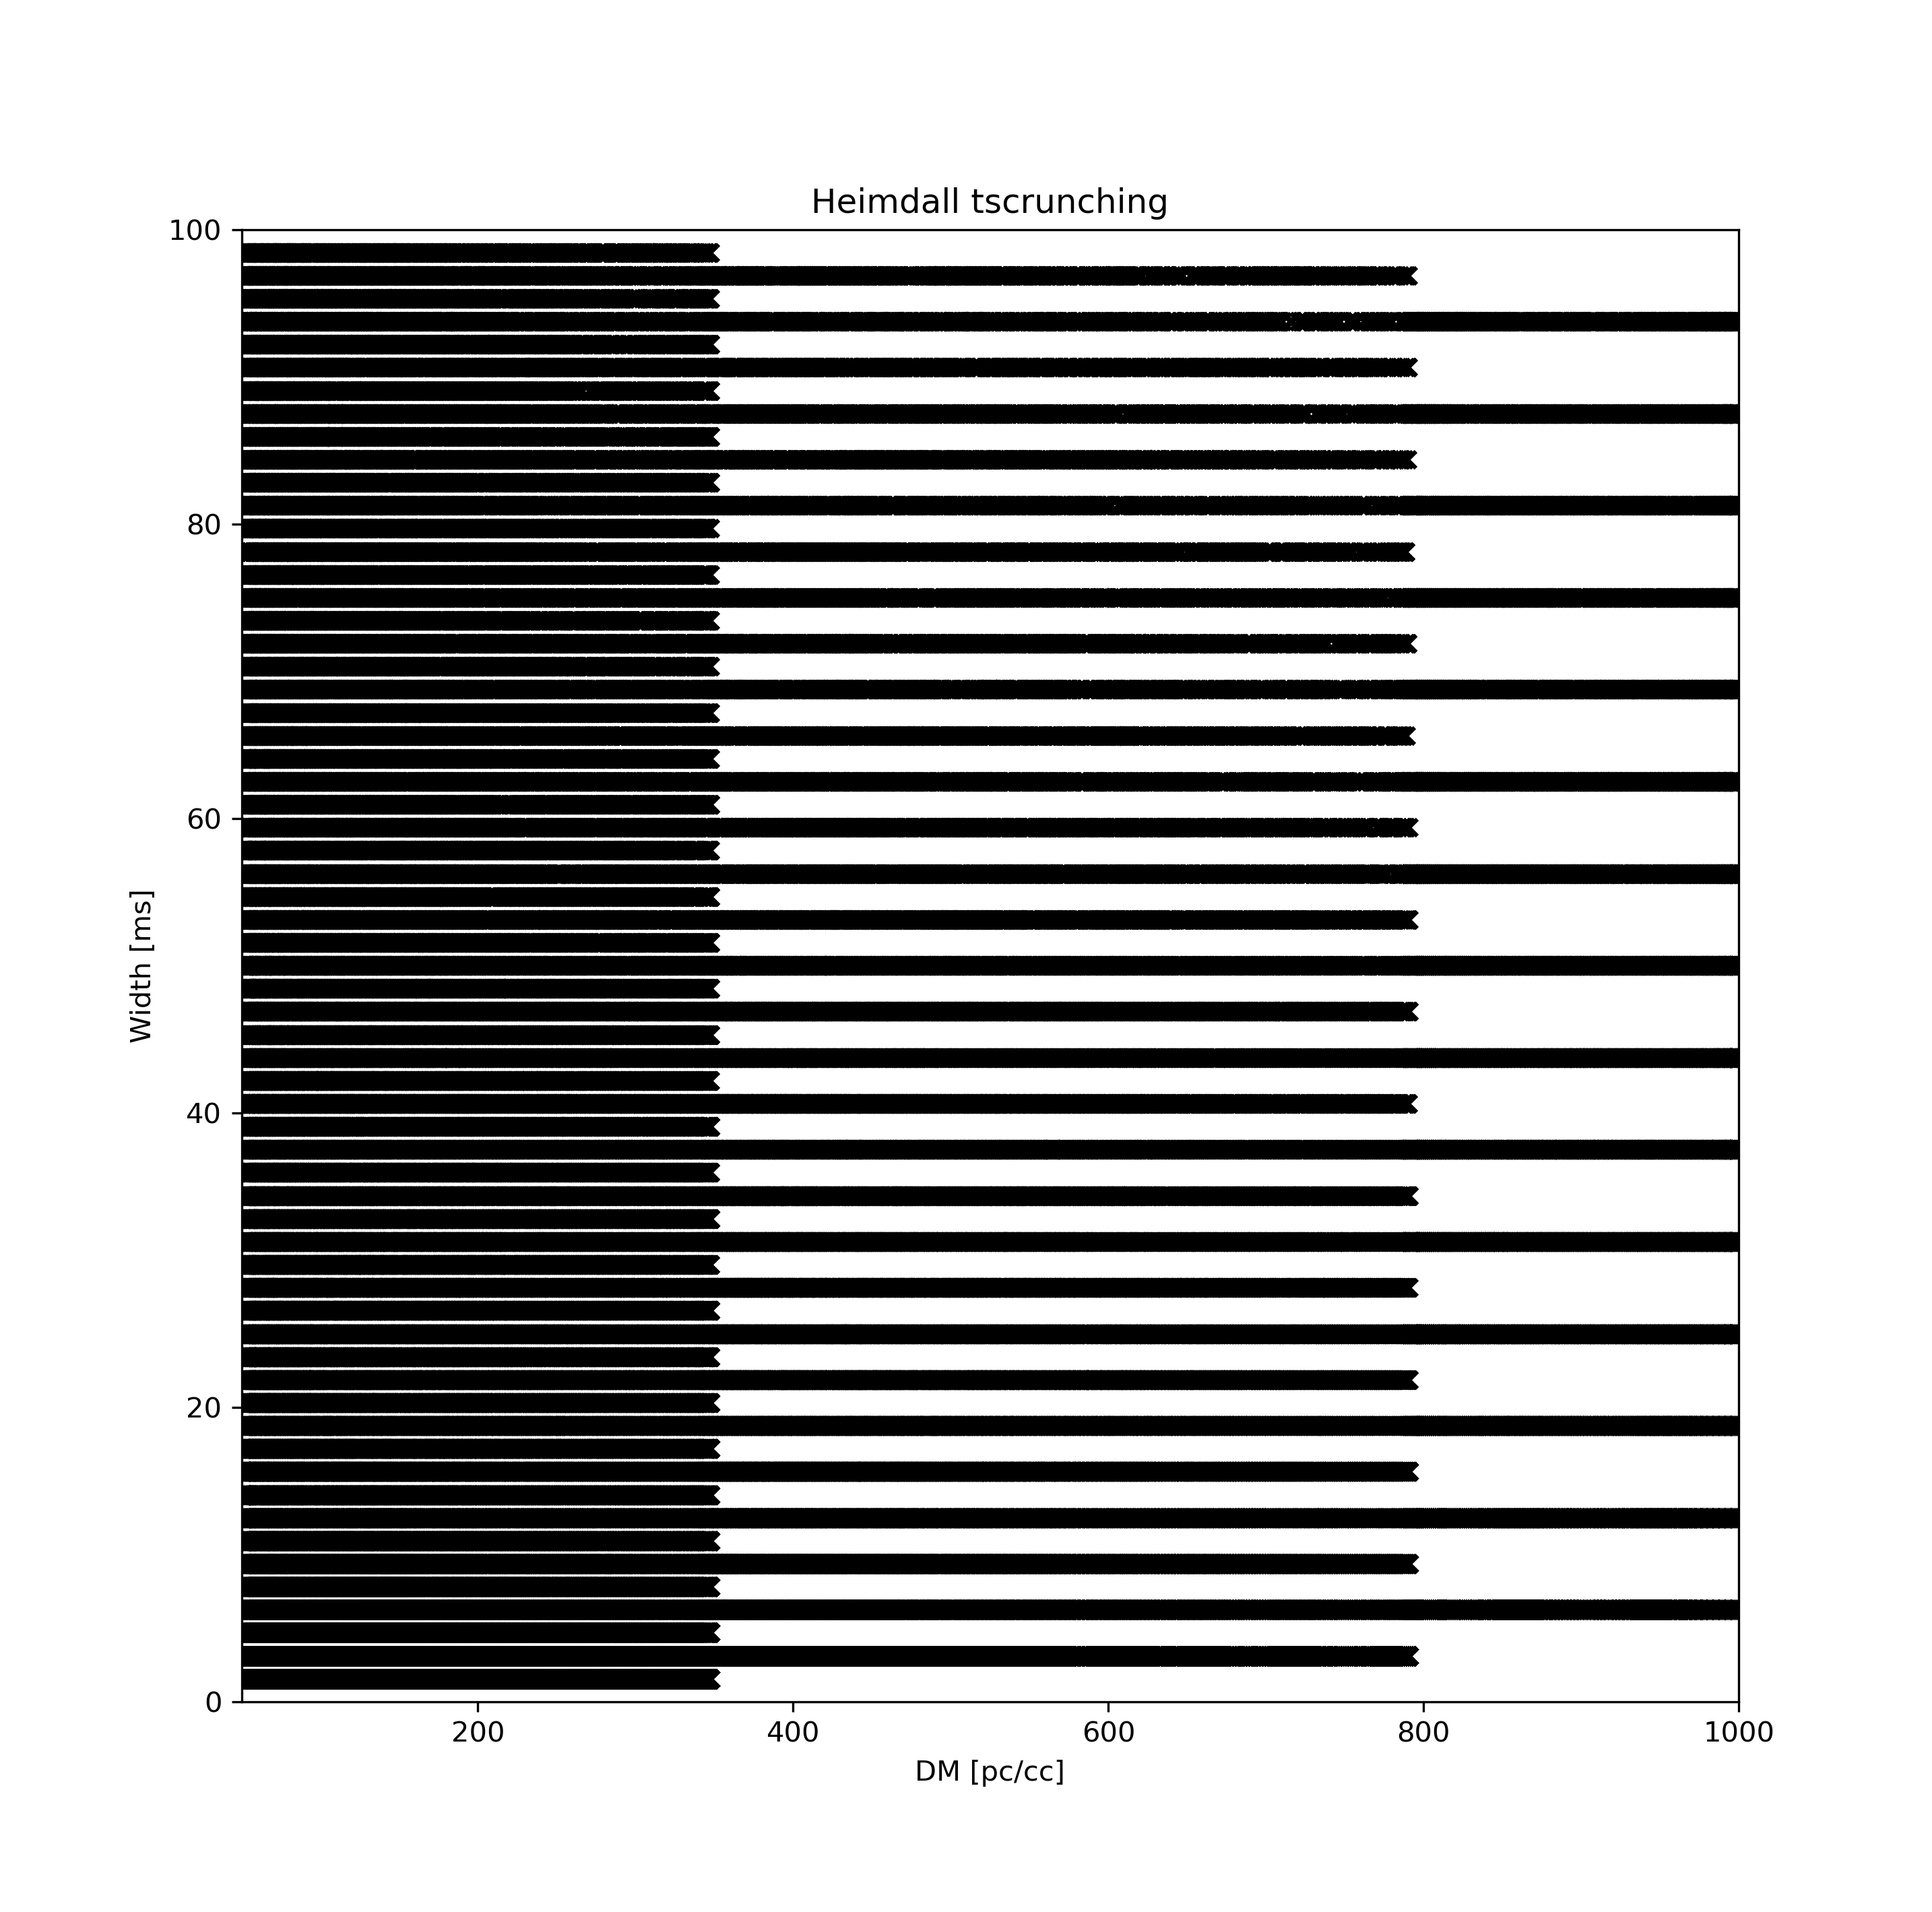
\includegraphics[width=0.8\textwidth, keepaspectratio]{heimquant.png}
	\caption{\dm-Width space of all the Heimdall triggers. Although the maximum width is set to $100$ ms, this plot only extends until $20$ ms.
		This space is expected to be uniform. The quantization seen in the width for large \dm is an affect of heimdall \emph{adaptive\_dt}.
	}
\end{figure}

\begin{figure}
	\label{fig:histdm}
	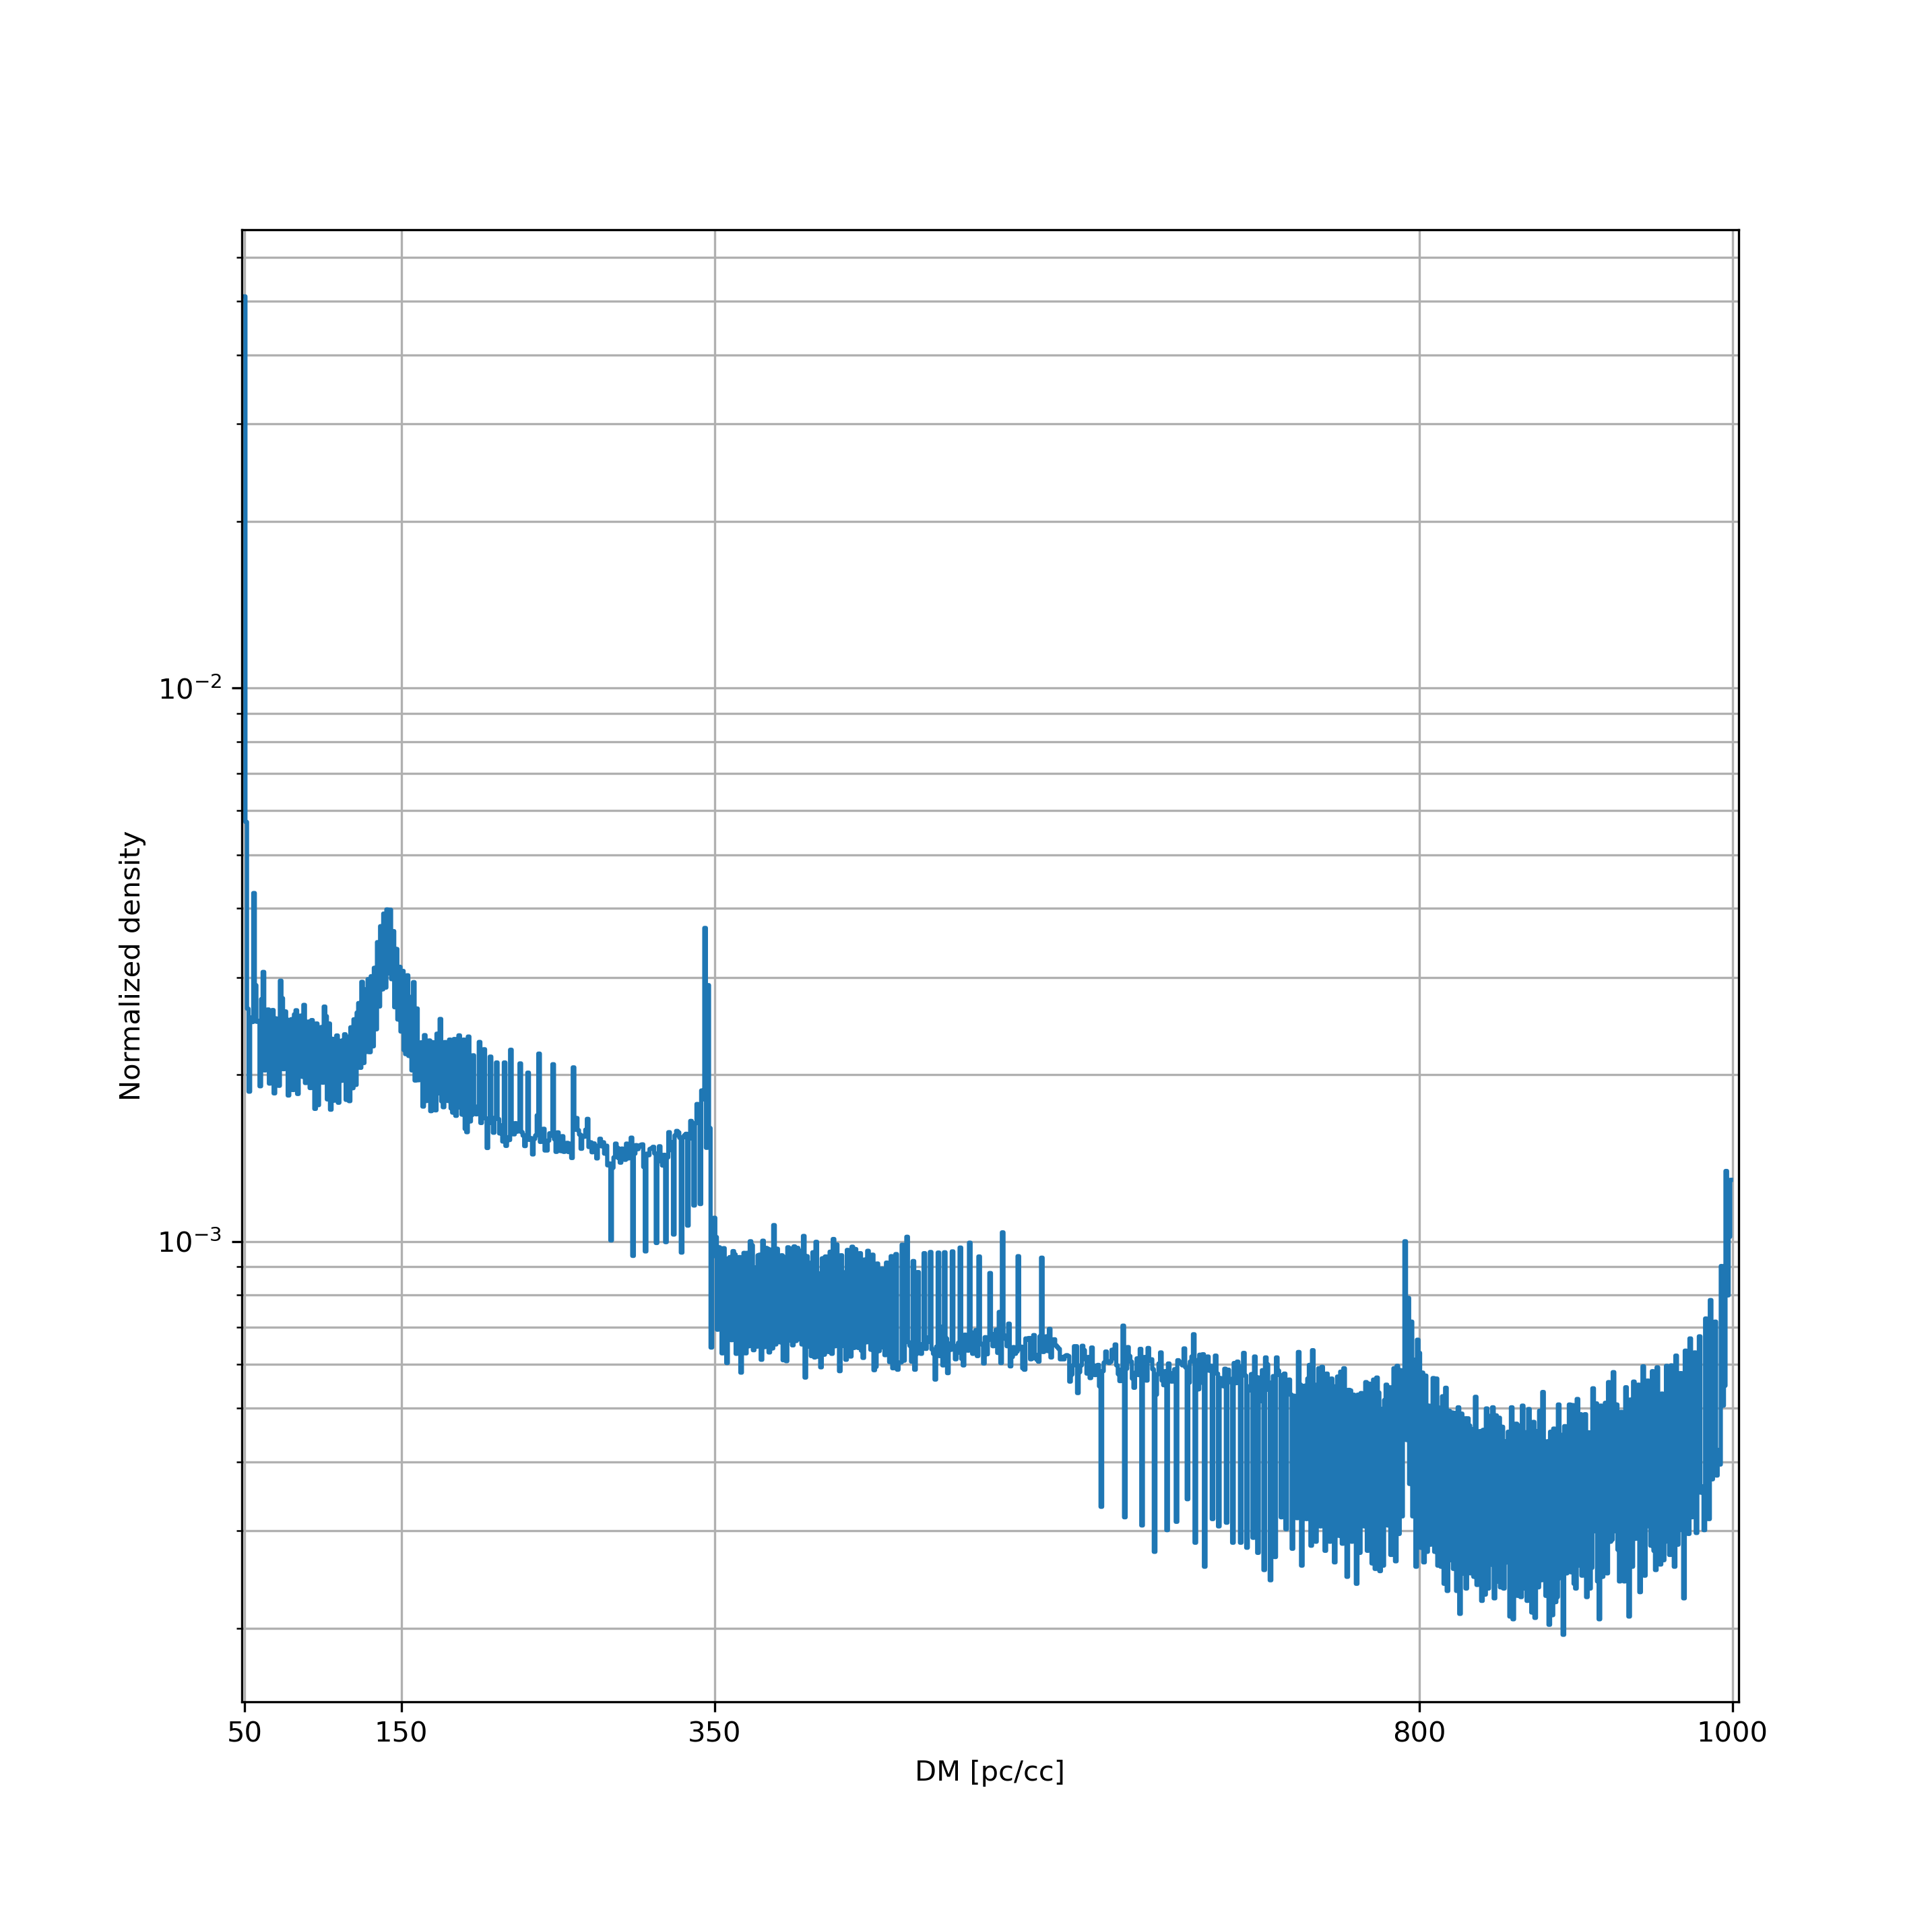
\includegraphics[width=0.8\textwidth, keepaspectratio]{dm_distro.png}
	\caption{Histogram of \dm of all the triggers recorded.
		The sharp line at \DM{50} is due to the \psr{J1752-2806}.
		The sharp lines at \DM{350}, \DM{800} and \DM{1000} are due to heimdall triband structure. See~\autoref{sec:htriband}.
		The very broad peak at \DM{150} is due to narrow band RFI. See~\autoref{ssub:dm150}.
	}
\end{figure}


\section{Summary statistics}
\label{sec:sum}
\par For a total uptime of $\sim 126$ days, the distribution of time spent on each pointing in shown in~\autoref{fig:skymap}.

\begin{figure}
	\centering
	\label{fig:skymap}
	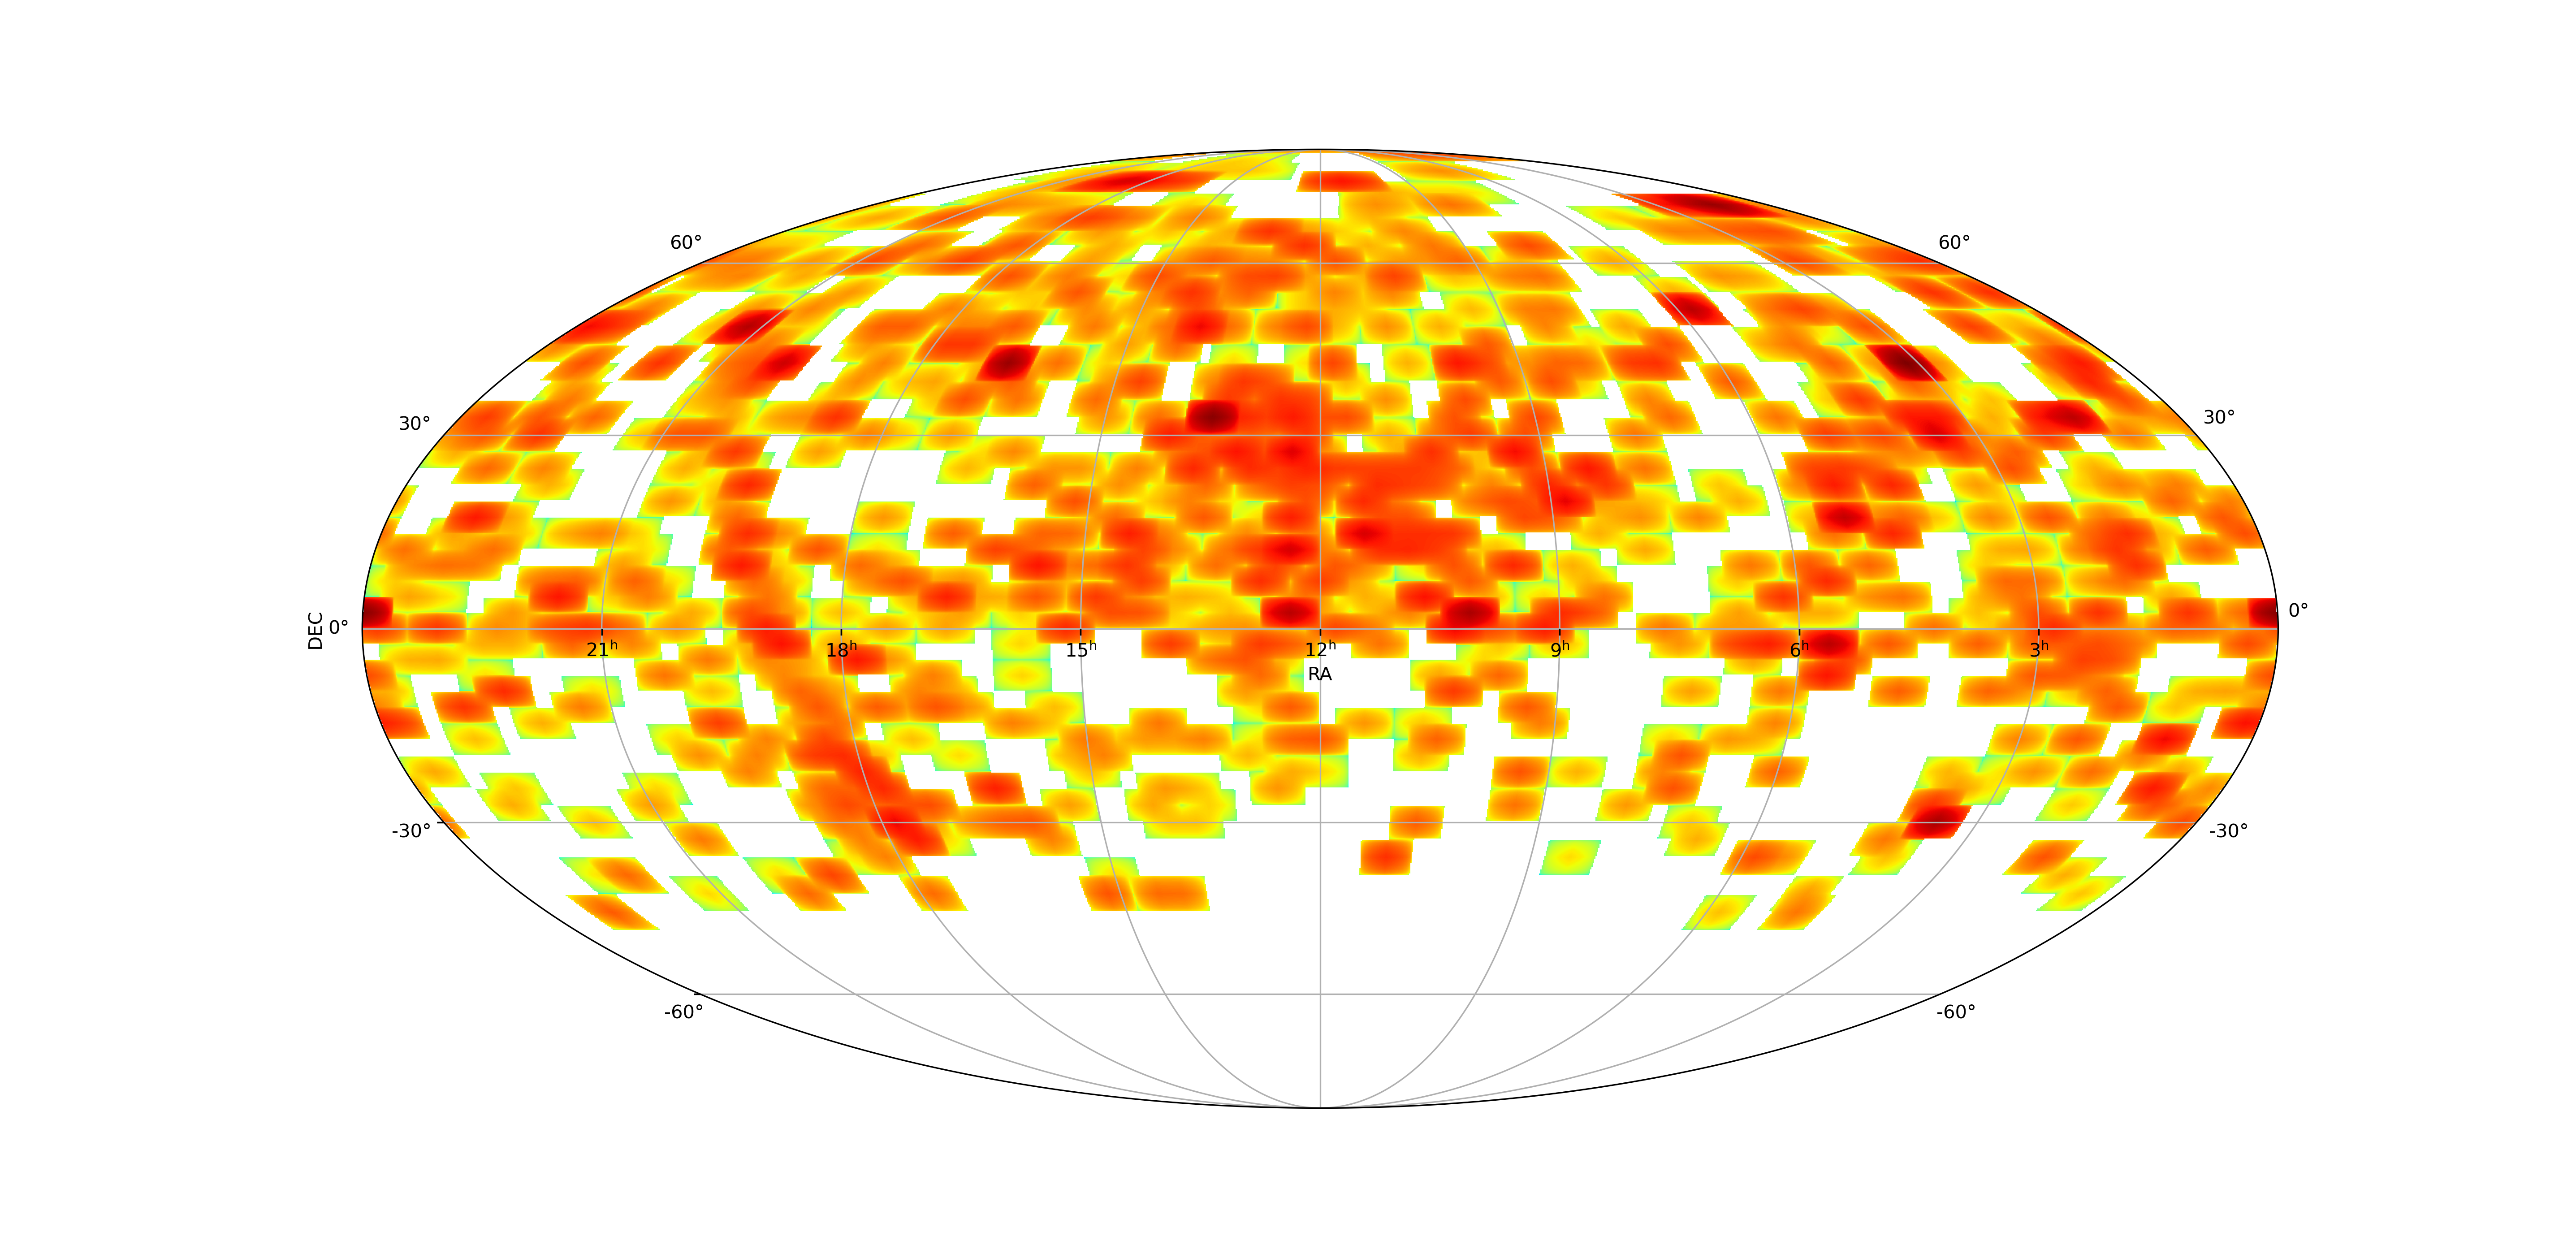
\includegraphics[width=0.8\textwidth, keepaspectratio]{g6m_skymap.png}
	\caption{Skymap of time spent on pointing in hours.}
\end{figure}


\section{Simulation runs}
\label{sec:sim}

\par In an effort to better understand the capabilities of \vf~, data was taken in controlled enviroments.
Those controlled environments and the results of the data taking are surmised here.

\subsection{Pure noise}
\par In this, \vf~data coming from the antennas was discarded and replaced with Gaussian random noise 
with mean $0$ and standard deviation $33.313$. 
Whatever triggers registered in such a run are purely noise triggers.
This simulation was run for $\sim 72$ hours collecting $\sim 10\ 000$ triggers.

\par The distribution of the \sn registered is in~\autoref{fig:wnrates}. The rates are tabulated for different \sn cuts in~\autoref{tab:wnrates}.

\begin{figure}
	\label{fig:wnrates}
	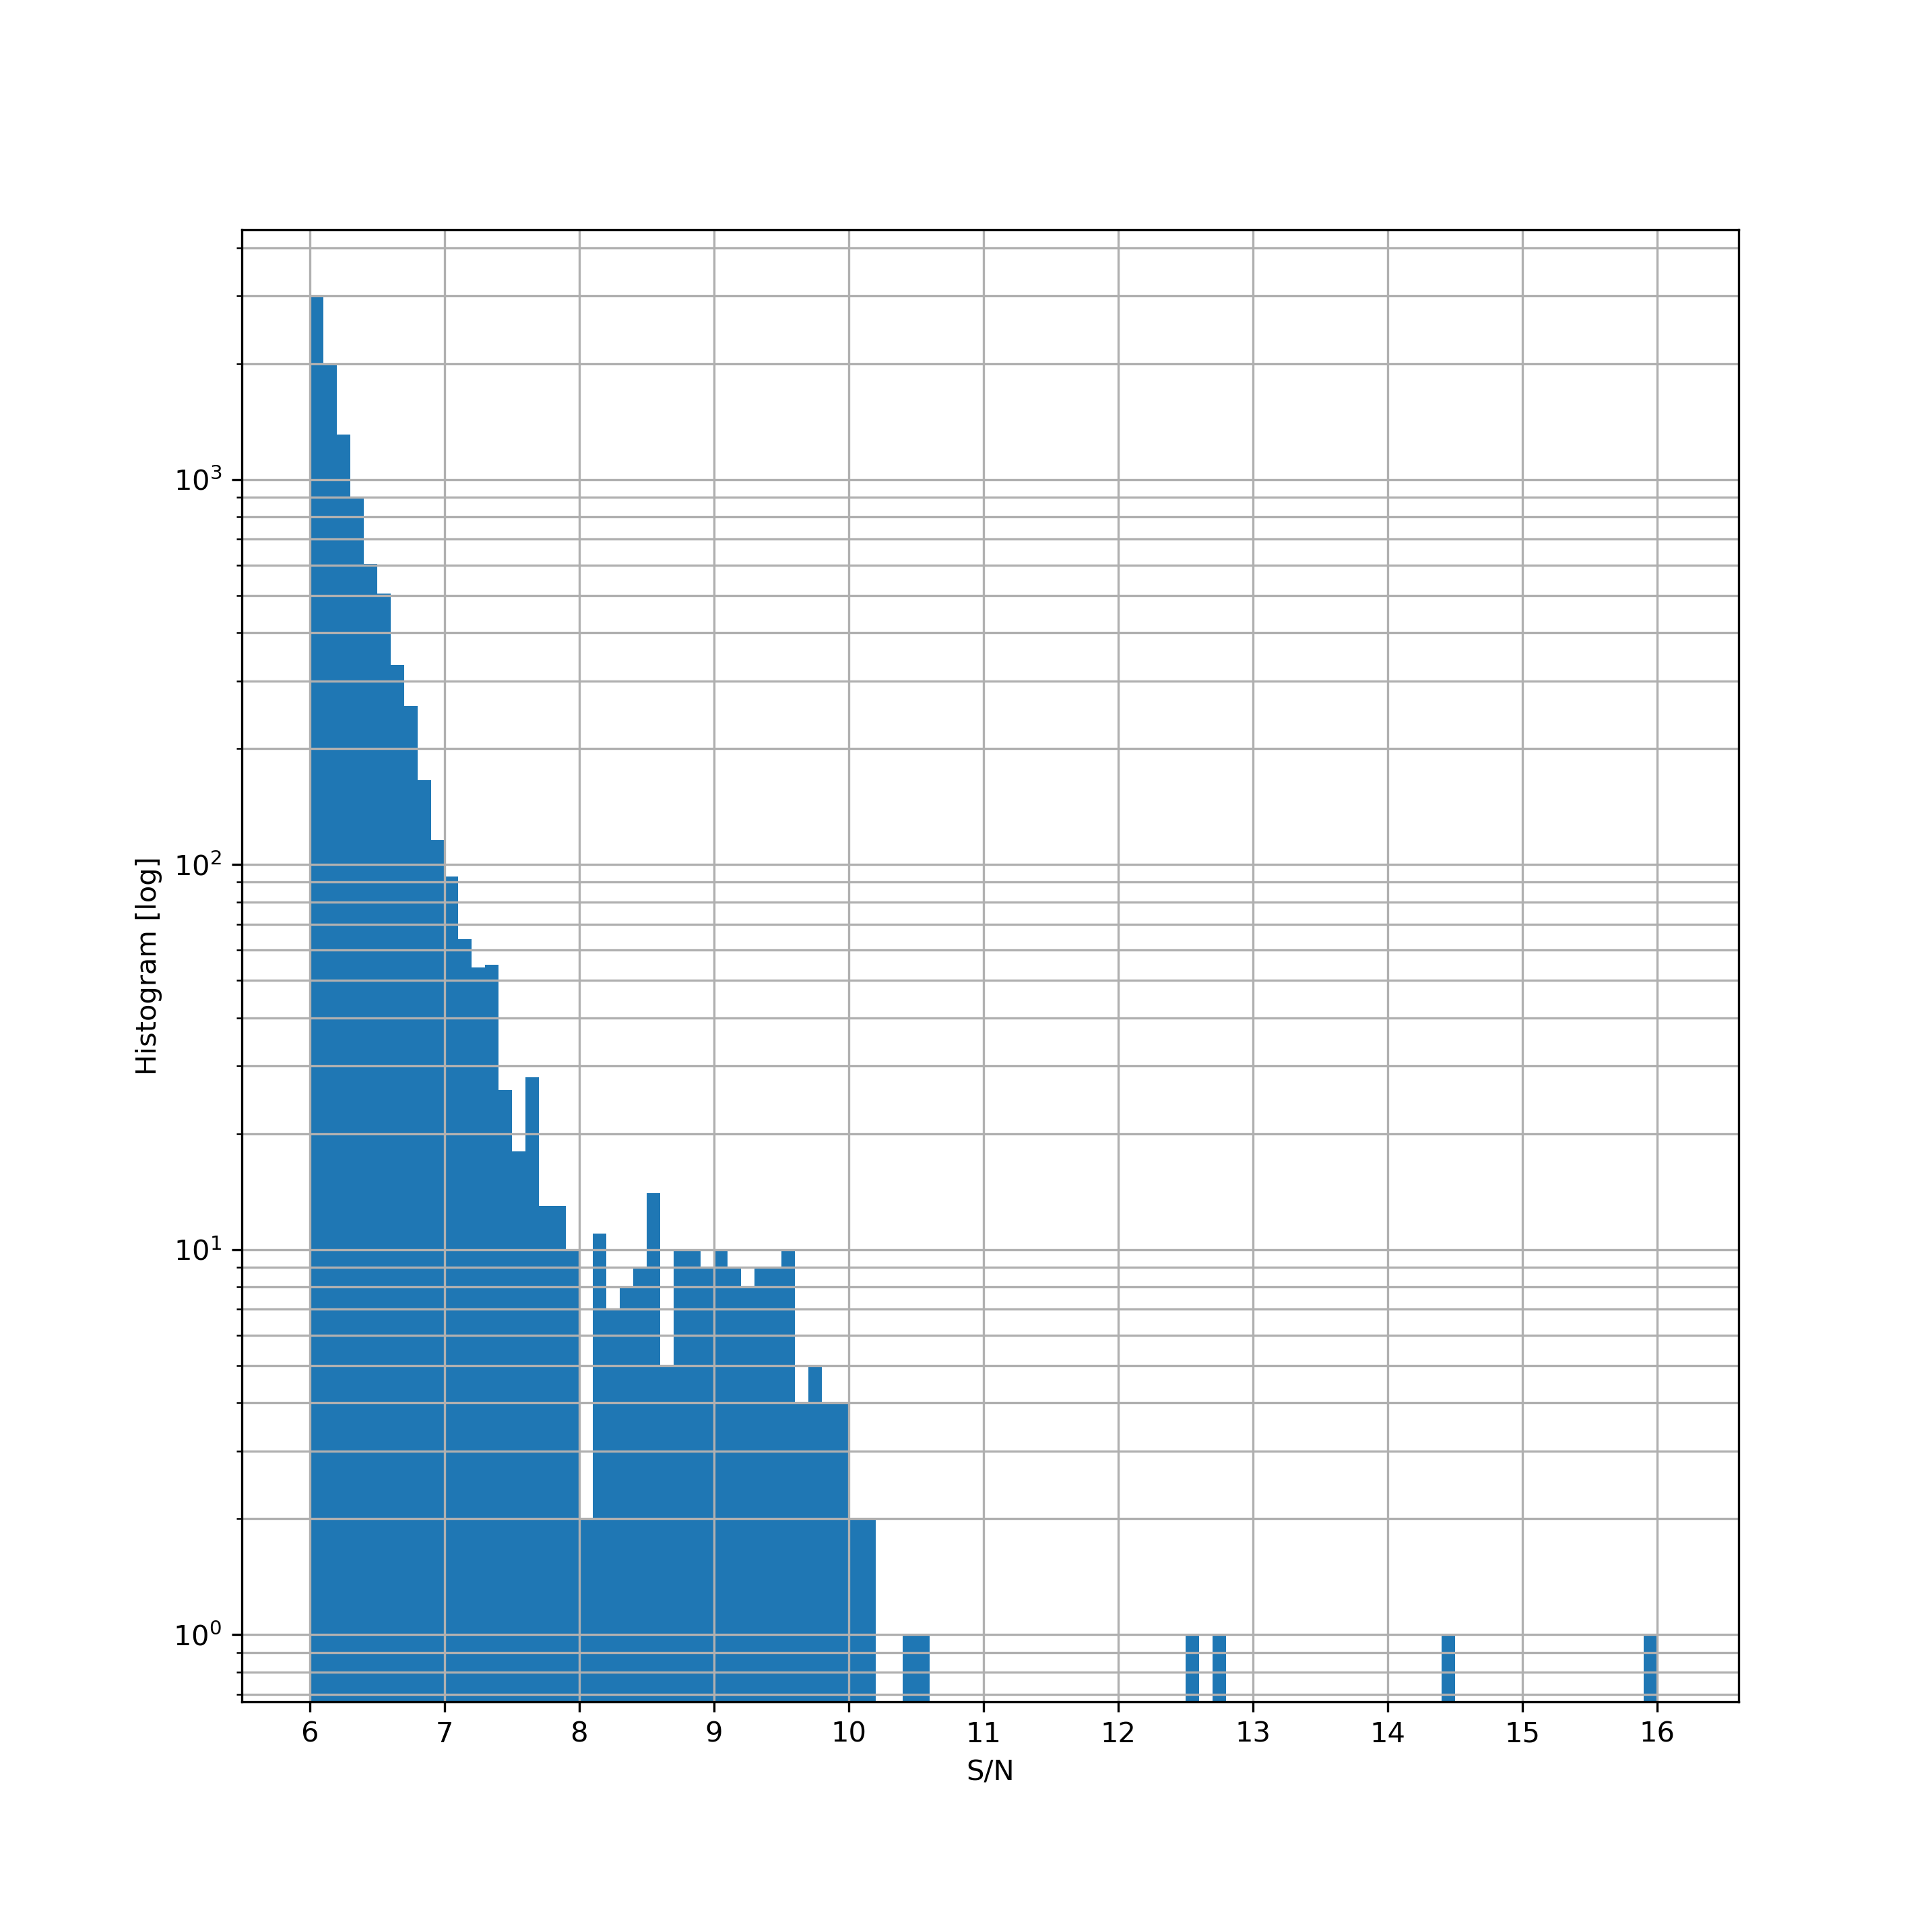
\includegraphics[width=0.8\textwidth, keepaspectratio]{histsnwn.png}
	\caption{Trigger rates observed at different \sn when only sending random noise through the pipeline.
		This figure shows how noise dominated lower \sn is. For low \sn ($6|8$), the relation is exponential.
		The valley seen at \SN{8} is result of changing trigger cuts used in dispatch in the MW campaign (See~\autoref{sec:camp}).
	}
\end{figure}

\par This exercise proved fruitful in understanding how the pipeline responds to pure noise.
Pure white noise has no signal content whatsoever. These triggers are result of pure noise data that looks exactly like a real single.
Thus is picked up by the pipeline. There is no technique, or procedure that can be applied to alleviate such triggers.
Hence are only argued upon in a statistical sense. See~\autoref{tab:wnrates}. 
The \sn cut in the MW run was $6$ which yielded a trigger rate of about $395$ hr$^{-1}$. 
This exercise shows that about $58\%$ of the triggers are due to pure random noise which is a lot.

% Please add the following required packages to your document preamble:
% \usepackage{booktabs}
\begin{table}[]
	\label{tab:wnrates}
	\begin{tabular}{@{}llll@{}}
		\toprule
		S/N cut & \begin{tabular}[c]{@{}l@{}}Trigger\\ rate (/hr)\end{tabular} & S/N cut & \begin{tabular}[c]{@{}l@{}}Trigger\\ rate (/hr)\end{tabular} \\ \midrule
		6 & 117.2 & 7.5 & 3 \\
		6.5 & 23.1 & 8 & 2 \\
		7 & 6.5 & 10 & 0.12 \\ \bottomrule
	\end{tabular}
	\caption{Trigger rates for different \sn cuts. Notice the extremely steep decline in trigger rate at low \sn. 
		This shows the extent of low \sn being whitenoise triggers. See text for more information.
	}
\end{table}


\subsection{Injected}
\par A dispersed signal of known \dm, amplitude, and \wd~ is added on top of random noise, and sent through the pipeline.
The signal is then recovered from the triggers collected.
This exercise shows how receptible \vf~pipeline is.
Since the known signal is embedded on top of random noise, there are also many noise triggers which are registered.
Such triggers are later filtered by comparing the time of injection with the time of trigger's peak.
\par This simulation run was designed to inject $15$ \frb{}s in $2$-minutes, yielding a trigger rate of $450$ hr$^{-1}$.
Due to the Heimdall tri-band structure (see~\autoref{htriband}), which makes the former less suspectible to high \dm triggers for widths far from the quantized width, the trigger rate captured was $308$ hr$^{-1}$.
~\autoref{fig:injected} shows four subplots. The triband structure is plotted in top left. The rest capture the distributions of registered \sn, \dm and widths.
\par The decreasing density for large \sn,\dm is because of Heimdall triband structure. 
Due to the quantization in the width for large \dm, many high \dm signals are not registered hence, a downward trend is observed in \sn, \dm.

\begin{figure}
	\label{fig:injected}
	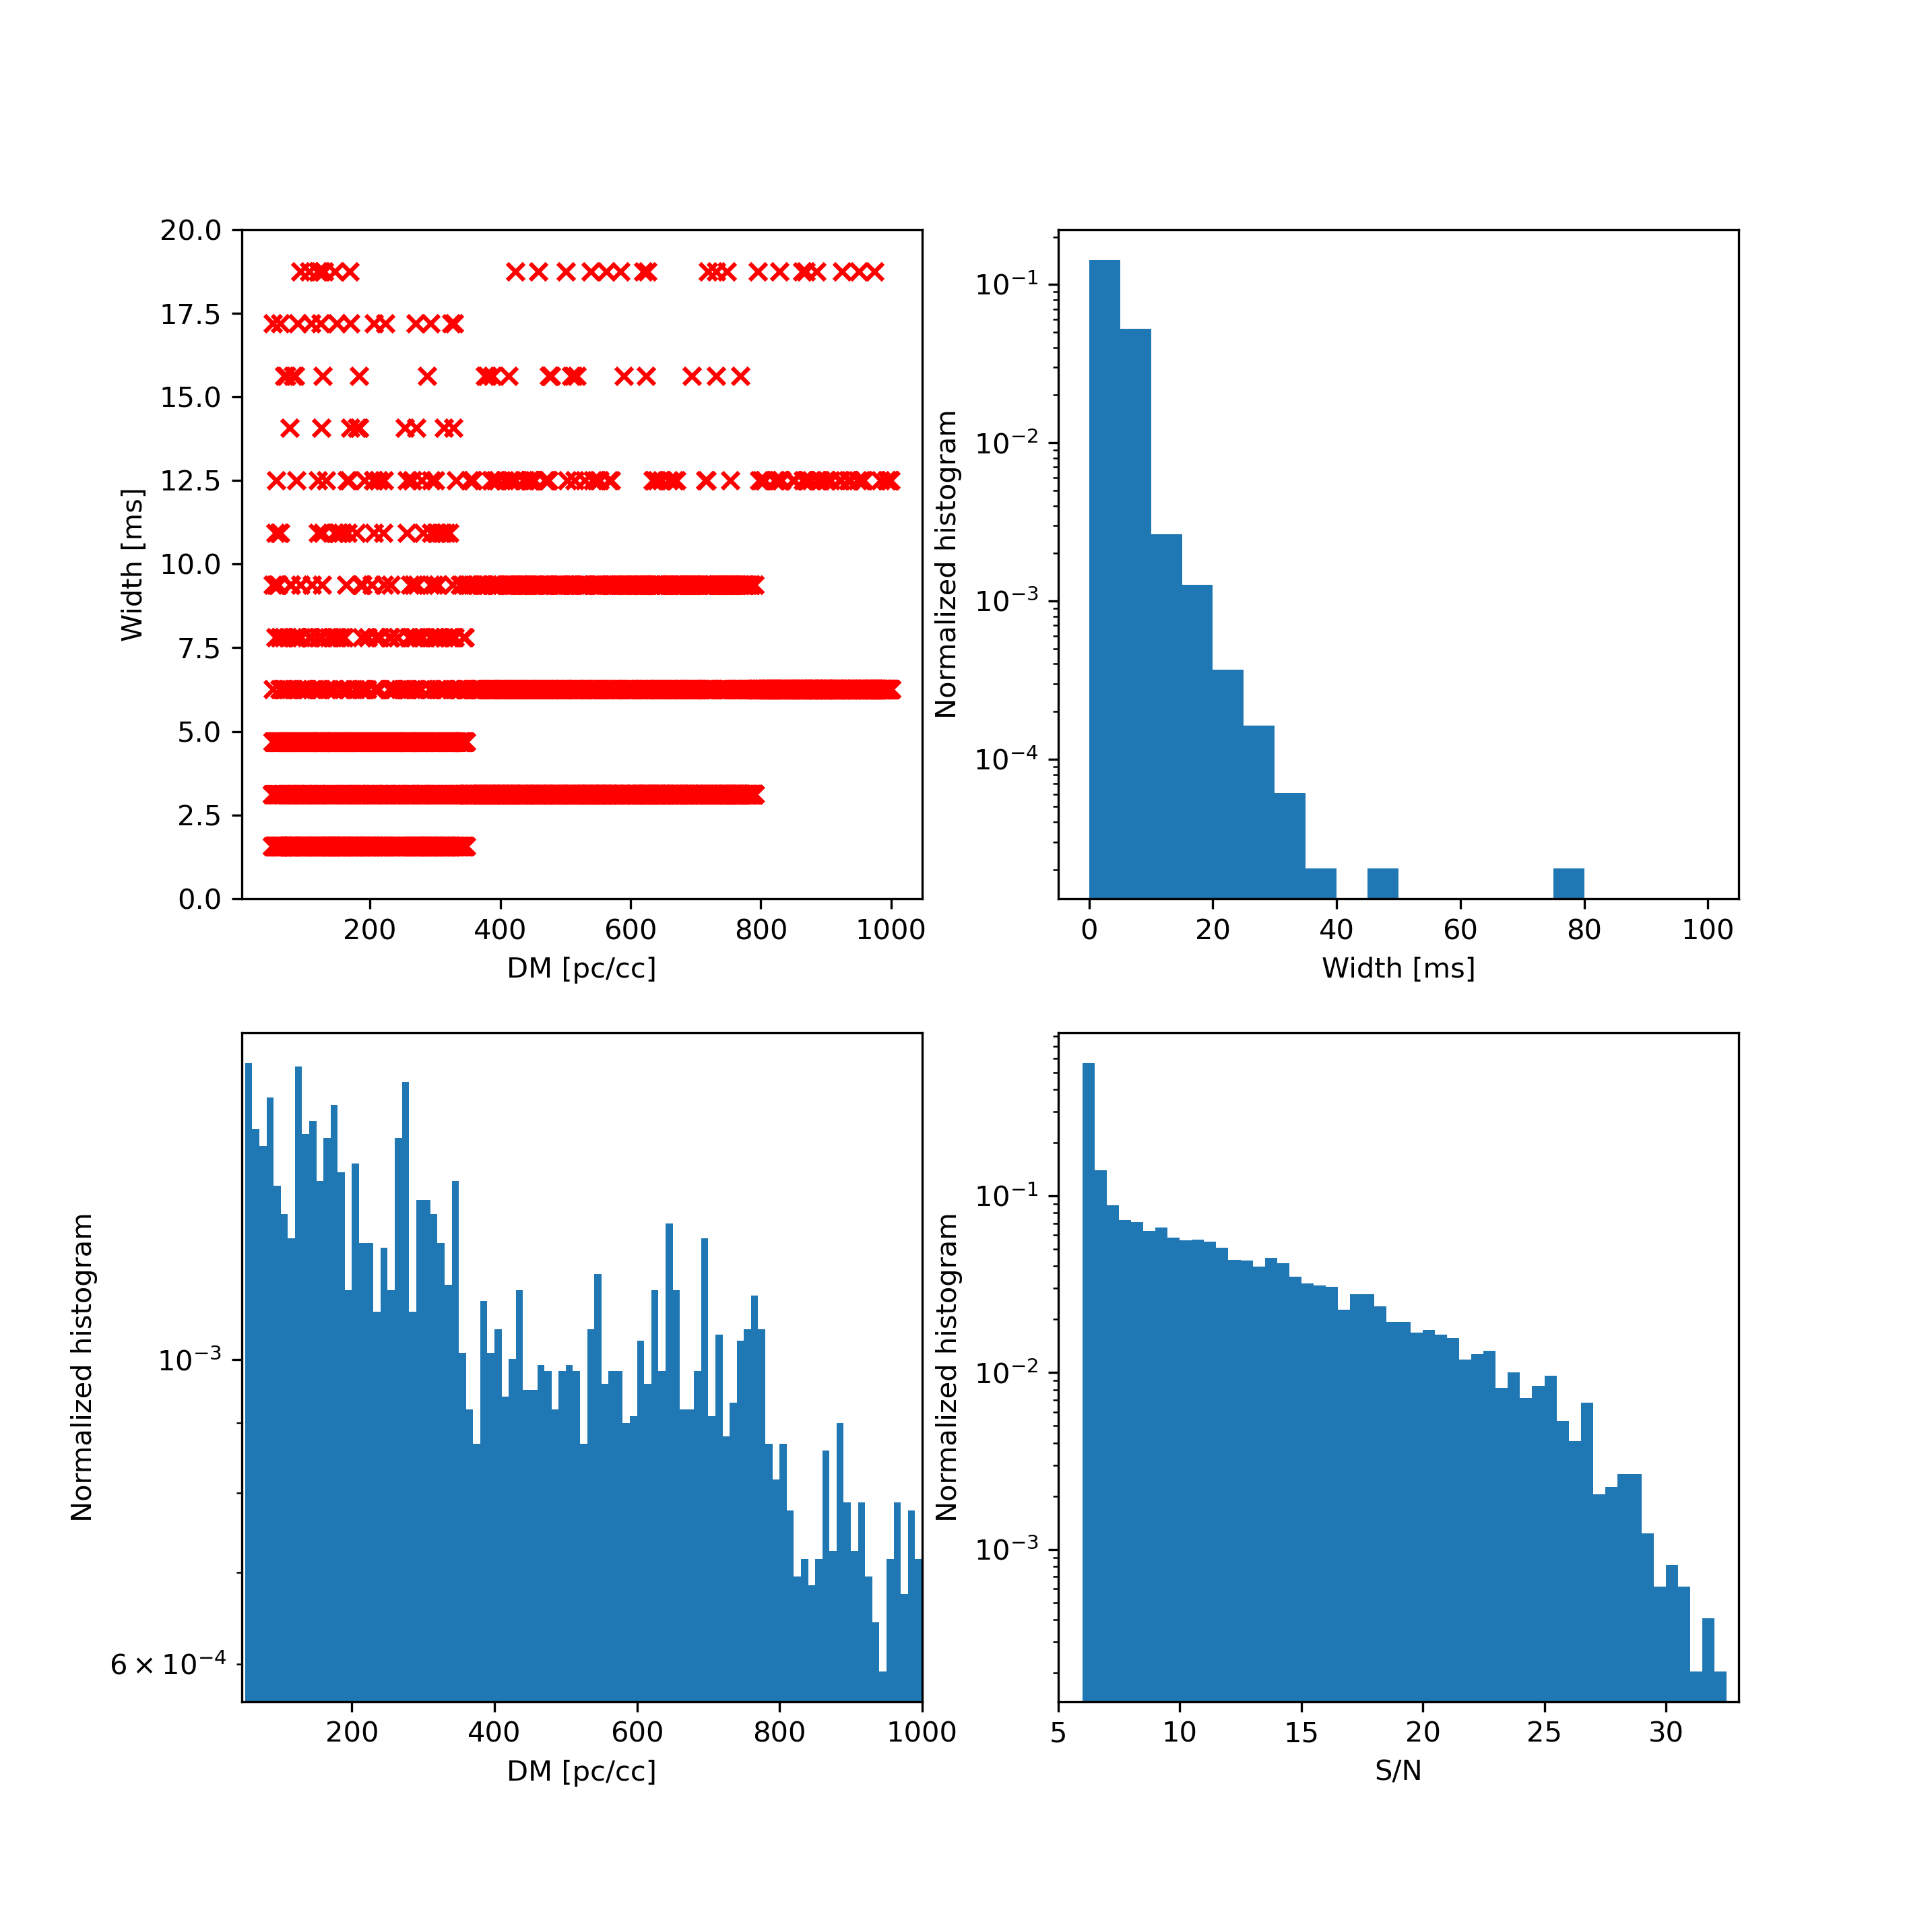
\includegraphics[width=0.8\textwidth, keepaspectratio]{injectedsub4.png}
	\caption{Top left: \dm v/s \wd showing quantization in \wd at high \dm consistent with triband structure (see text in~\autoref{sec:htriband})
		Top right: Distribution of registered width.
		Bottom left: Distribution of registered \dm.
		Bottom right: Distribution of registered sn.
		Injections parameters are derived from a uniform distribution and the same is expected in the registered \sn, \dm and widths.
		However, due to the triband structure, it is not achieved. The drop in density at high \sn is attributed to some percentage of injected triggers (high \dm) are failed to register.
	}
\end{figure}
